\section{Analysis}

%Analysis may involve: Interpretation, Presentation, comparison and confirmation

% The analysis chapter will present and discuss the main findings and outcomes, with limits being acknowledged (ie. Survey response levels, generalisability of results, reliability of tests, factos outwith your control.)

\subsection{Data analysis}

% Outline key variables and hypostheses being tested. 
The accuracy, precision, recall and numbers of probes sent will be used as the basis of establishing performance of the contemporary methods. This data is quantitative, with accuracy, precision and recall being continuous and number of probes sent discrete. 

Furthermore, side by side visual comparison between the simulated network topology and the measured network topology will also be presented. This data is categorical and is also binary, due to the compared topologies either being equivalent or not. 

% Data collection
The data will be collected through experimentation in a virtual network lab, as outlined above. Measurement of each configuration will be repeated five times, in order to ensure the validity of the results and allow for statistical analysis. 

% Data preparation
The network topology structure is pre-defined inside a YAML configuration file. Whereby the topology is defined in a set of \textit{nodes} and the \textit{links} between given nodes. Each node has a given \textit{kind} and \textit{image}, with the kind defining the node configuration and behaviour. Each node also has an \textit{image}, which defines the operating system which is to be ran on a given node. Each \textit{link} is defined through an array of end-points between each node. 

% Tools/Mathimatical models used for analysis
Experimental data will be exported in JSON format, from which it can be easily processed. The mean, mode, median and standard deviation will be presented for each finding. Analysis of the implemented model will be carried out using several metrics in order to illustrate comparisons between it's performance and the original model's performance. Several plot types such as scatter plots, line plots and violin plots will be used to visualize; negative and positive correlations and also to represent the standard deviation of results respectively. Furthermore, tables of data will also be used to provide accurate numerical data in a straightforward manner.

% 6. Connect methods to research objectives

%focusing on the study, hypothesis, sample groups you wish to address, and the limitations you have faced.

\subsection{Results}


\subsubsection{Topology set 1}
As shown from the comparison between the Erdos-Renyi, Barabasi-Albert, and real-world topologies, Janet and Napnet; the Erods-Renyi has the closest distribution of shortest path lengths to the real-world topologies. It also shows the effect that changing the $p$, parameter has, with 0.2 being the optimal value out of the measured parameters. 

\begin{figure}
    \centering
    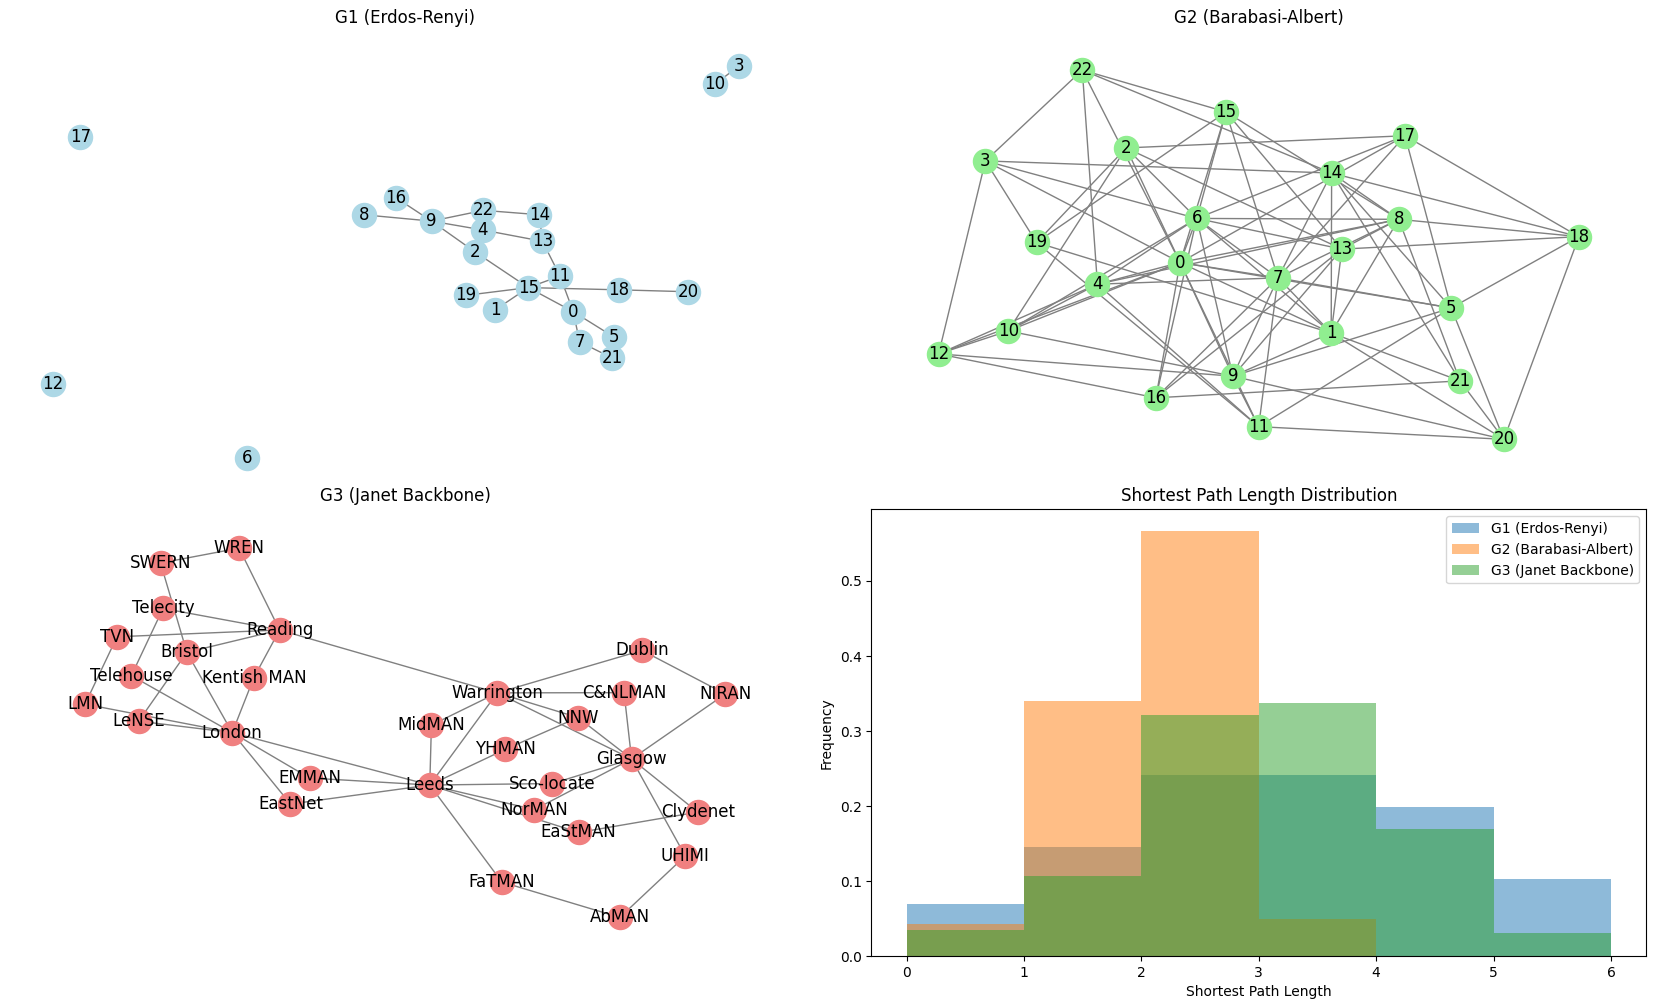
\includegraphics[width=0.7\linewidth]{images/final-topo-comparison/1_1.png}
    \caption{Erdos-Renyi (23 nodes,p=0.1), Barabasi-Albert(23 nodes, 5) and Janet-Backbone topology comparison}
    \label{fig:1_1_comparison}
\end{figure}

\begin{figure}
    \centering
    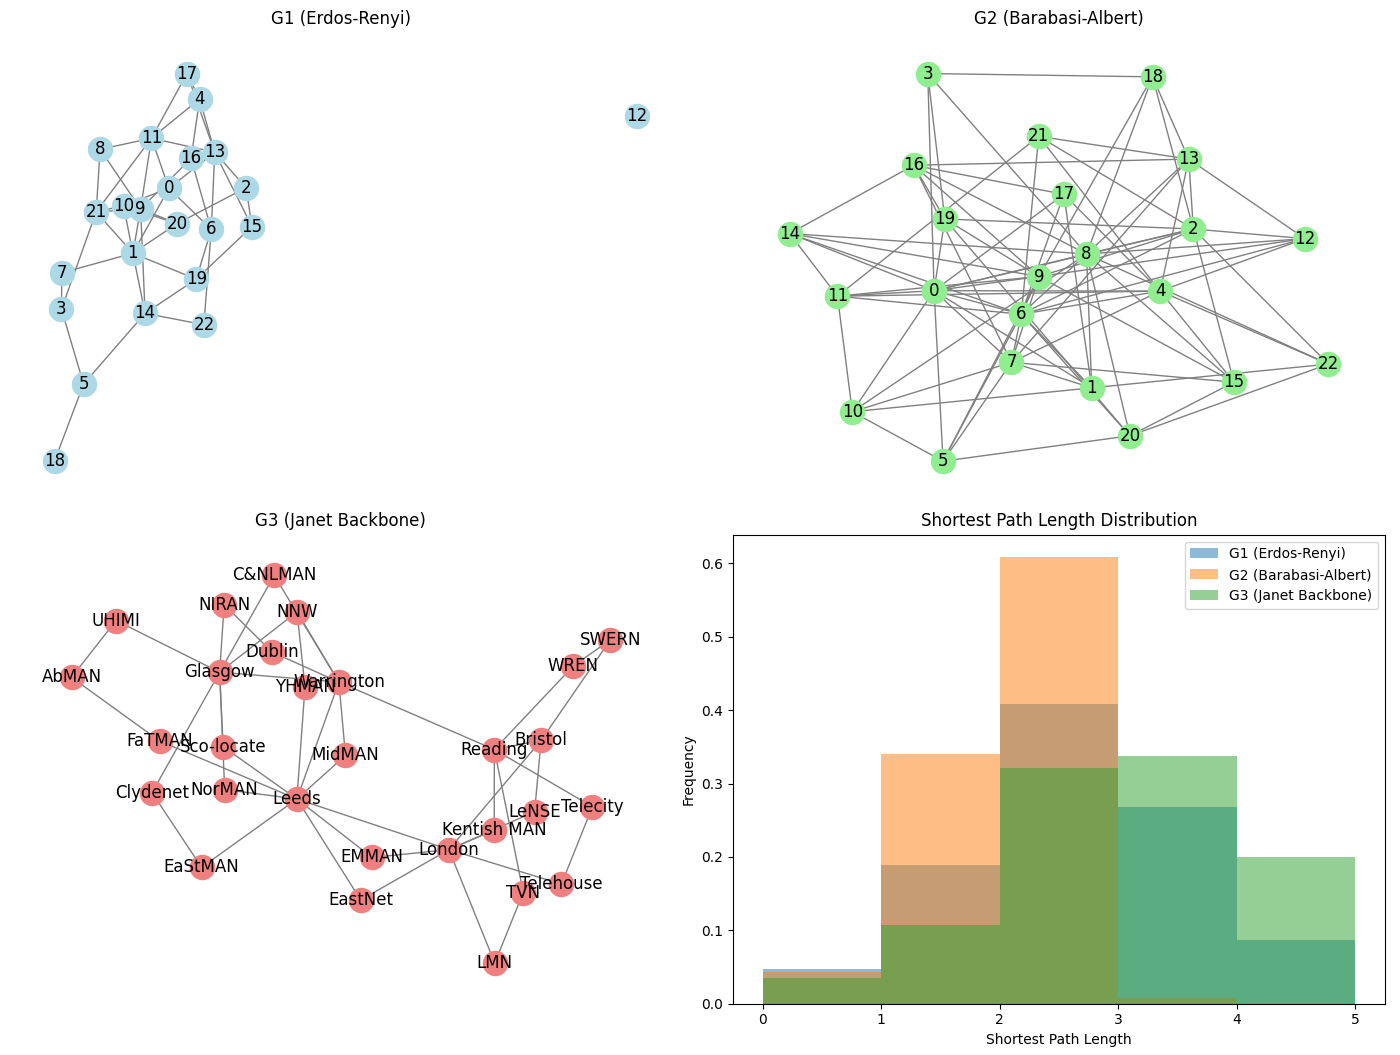
\includegraphics[width=0.7\linewidth]{images/final-topo-comparison/2_1.png}
    \caption{Erdos-Renyi (23 nodes,p=0.2), Barabasi-Albert(23 nodes, 5) and Janet-Backbone topology comparison}
    \label{fig:2_1_comparison}
\end{figure}

\begin{figure}
    \centering
    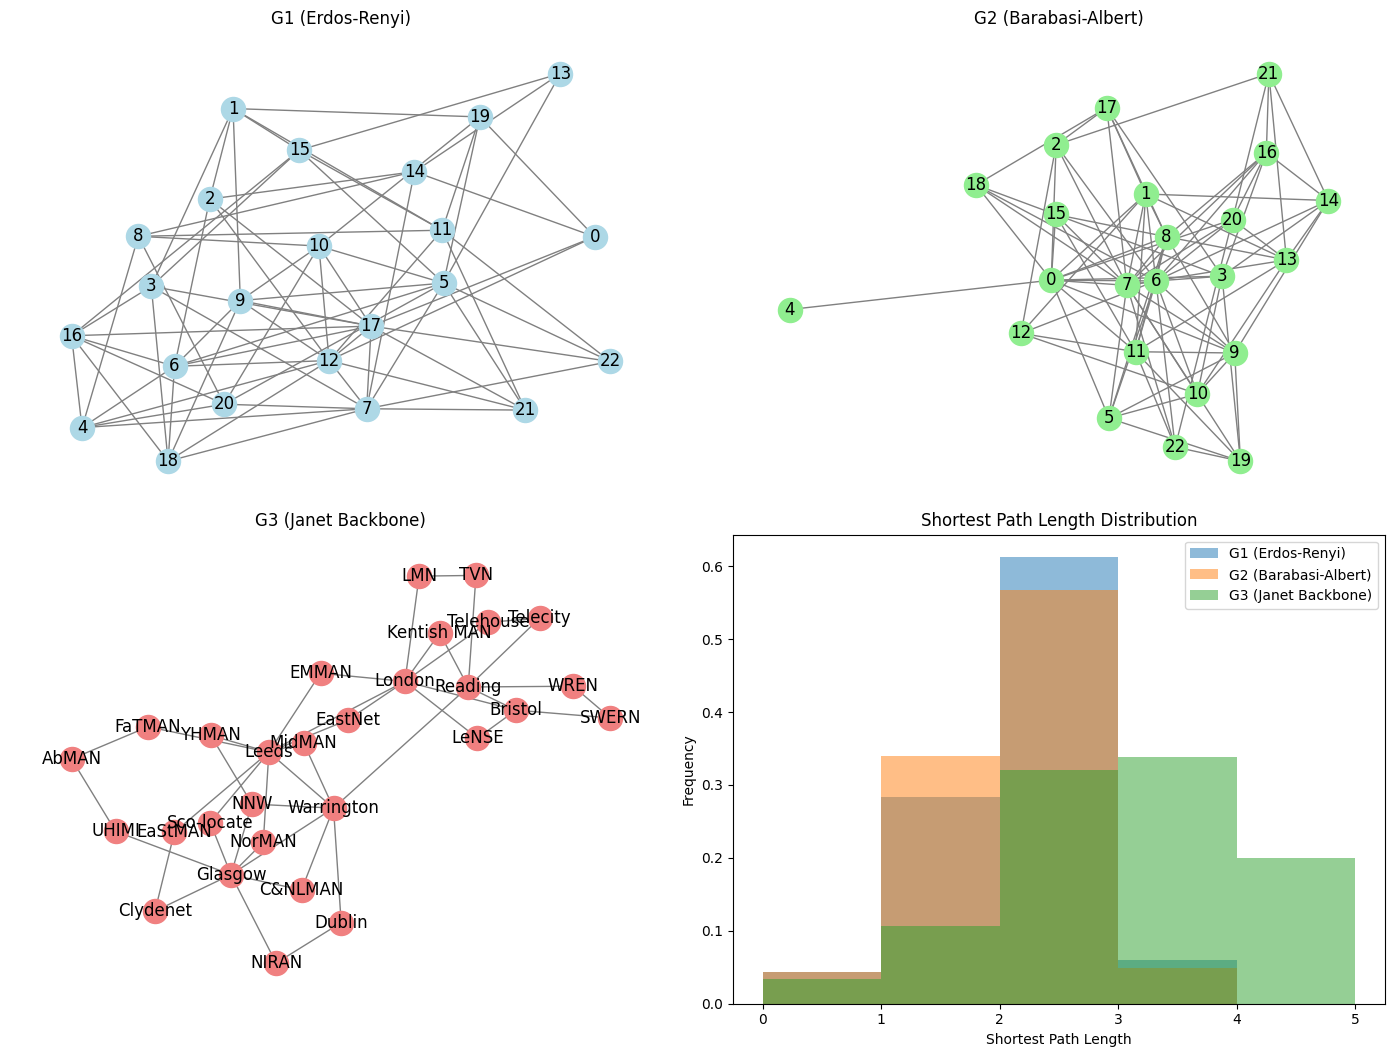
\includegraphics[width=0.7\linewidth]{images/final-topo-comparison/3_1.png}
    \caption{Erdos-Renyi (23 nodes,p=0.3), Barabasi-Albert(23 nodes, 5) and Janet-Backbone topology comparison}
    \label{fig:3_1_comparison}
\end{figure}

\newpage

\begin{figure}
    \centering
    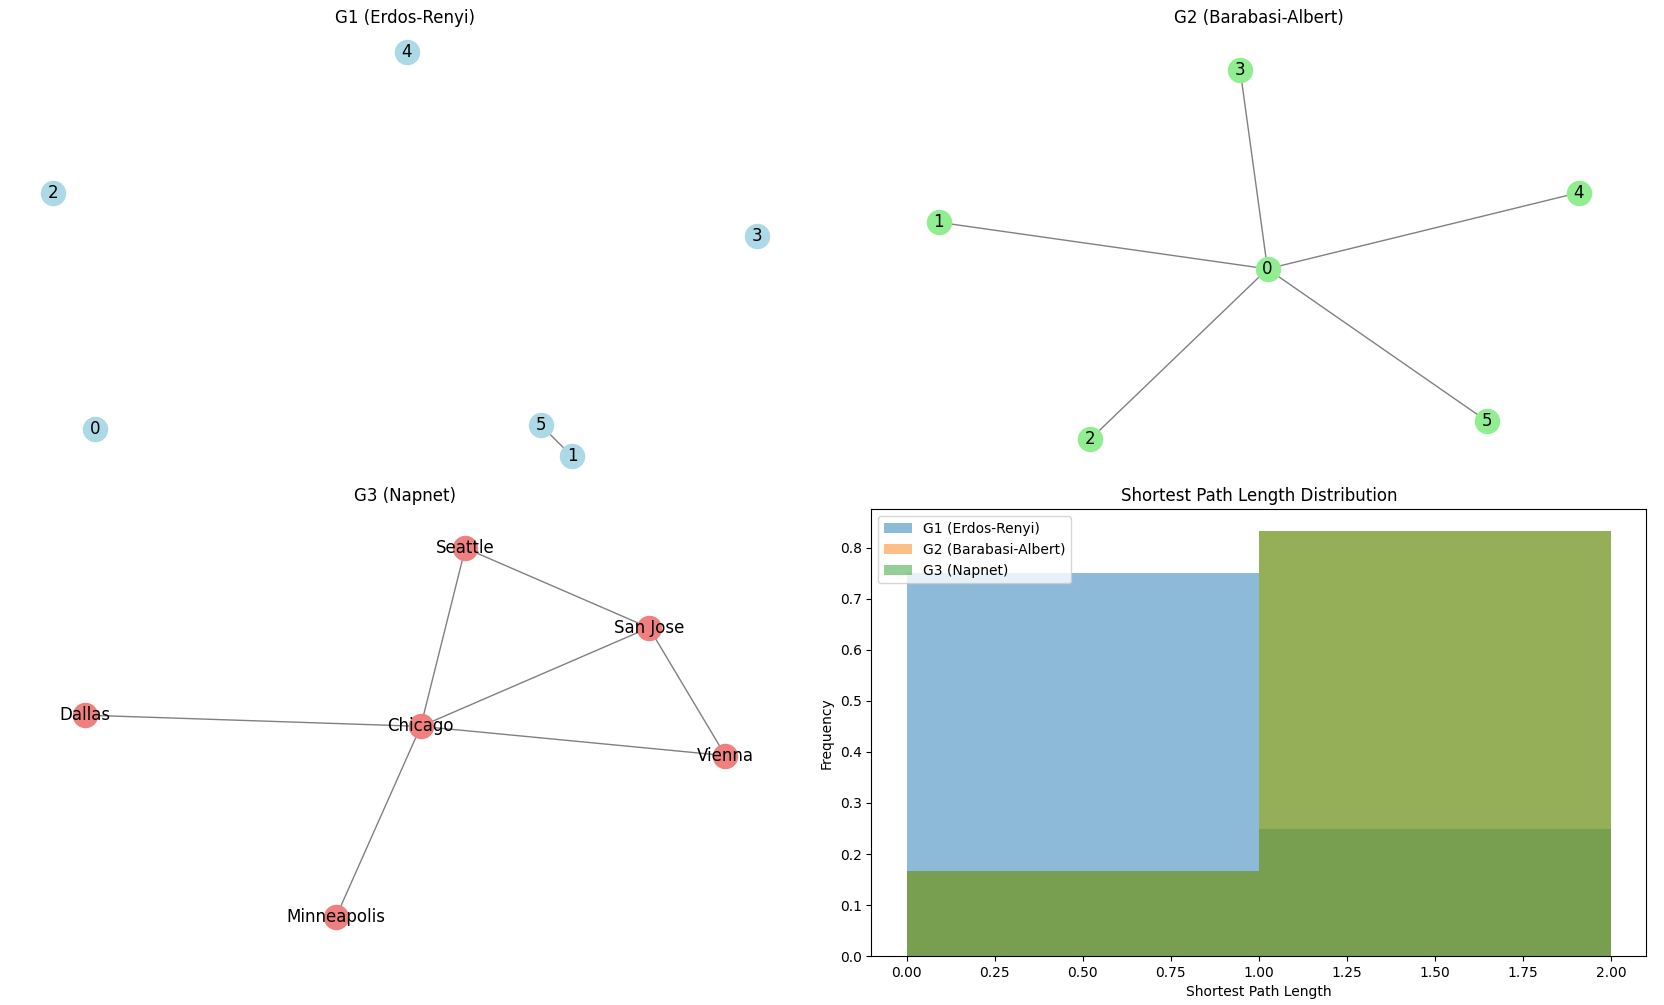
\includegraphics[width=0.7\linewidth]{images/final-topo-comparison/napnet/1_1.png}
    \caption{Erdos-Renyi (5 nodes,p=0.1), Barabasi-Albert(5 nodes, 5) and Napnet topology comparison}
    \label{fig:napnet_1}
\end{figure}

\begin{figure}
    \centering
    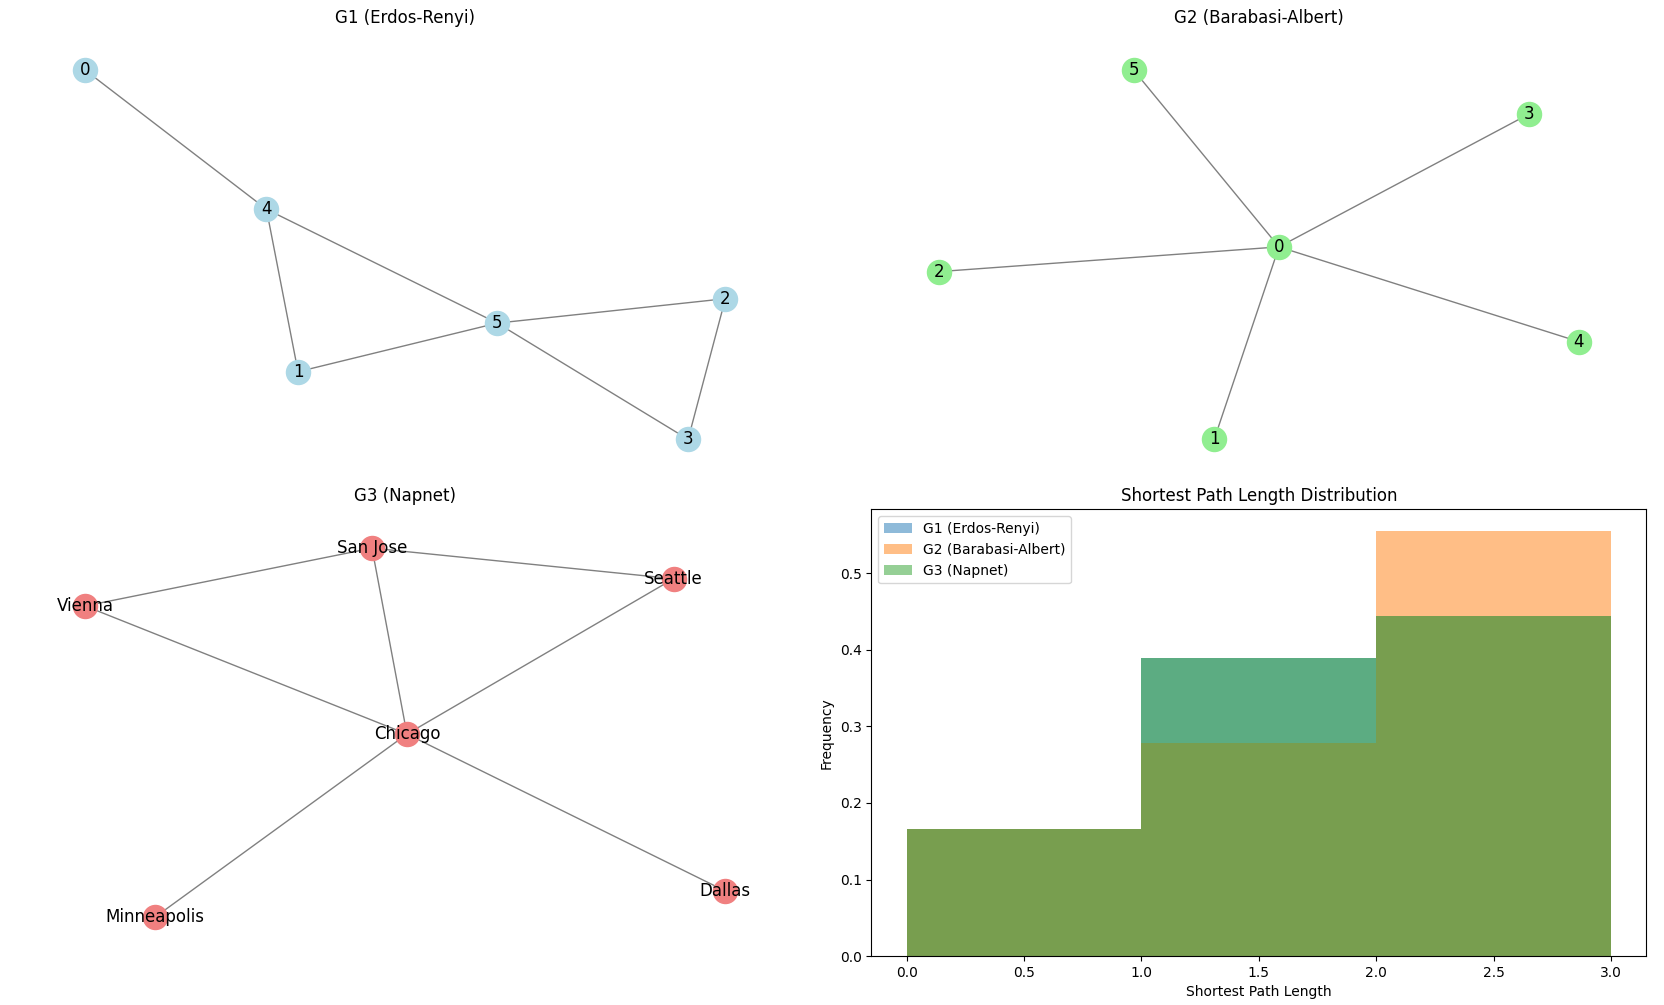
\includegraphics[width=0.7\linewidth]{images/final-topo-comparison/napnet/2_1.png}
    \caption{Erdos-Renyi (5 nodes,p=0.2), Barabasi-Albert(5 nodes, 5) and Napnet topology comparison}
    \label{fig:napnet_2}
\end{figure}

\begin{figure}
    \centering
    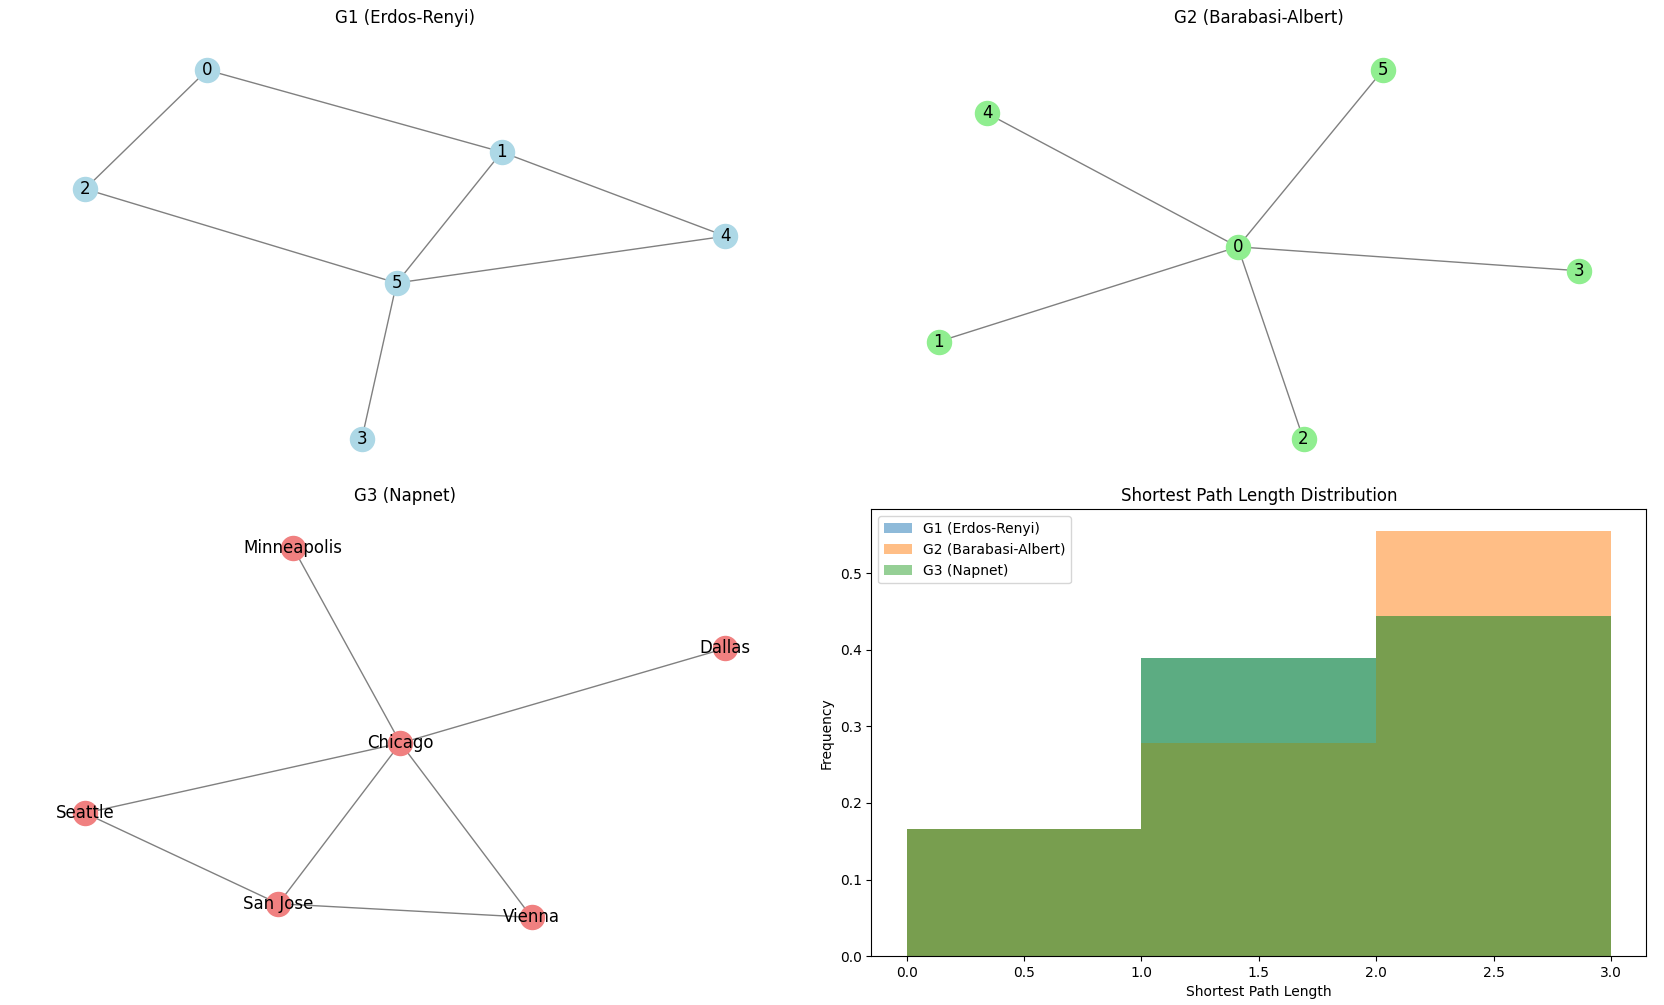
\includegraphics[width=0.7\linewidth]{images/final-topo-comparison/napnet/3_1.png}
    \caption{Erdos-Renyi (5 nodes,p=0.3), Barabasi-Albert(5 nodes, 5) and Napnet topology comparison}
    \label{fig:napnet_3}
\end{figure}

\subsubsection{Topology set 2}
\subsection{Topology set 3}

\subsection{Evaluation of Results}